\section{Fundamental knowledge}
% =========================================
% =========================================

\begin{frame}{Fundamental knowledge for modeling}
	\framesubtitle{Coordinates}
	
	
	\begin{tikzpicture}[remember picture,overlay]
		\node at (current page.north east) [xshift=-3.5cm, yshift=-4.7cm] 
		{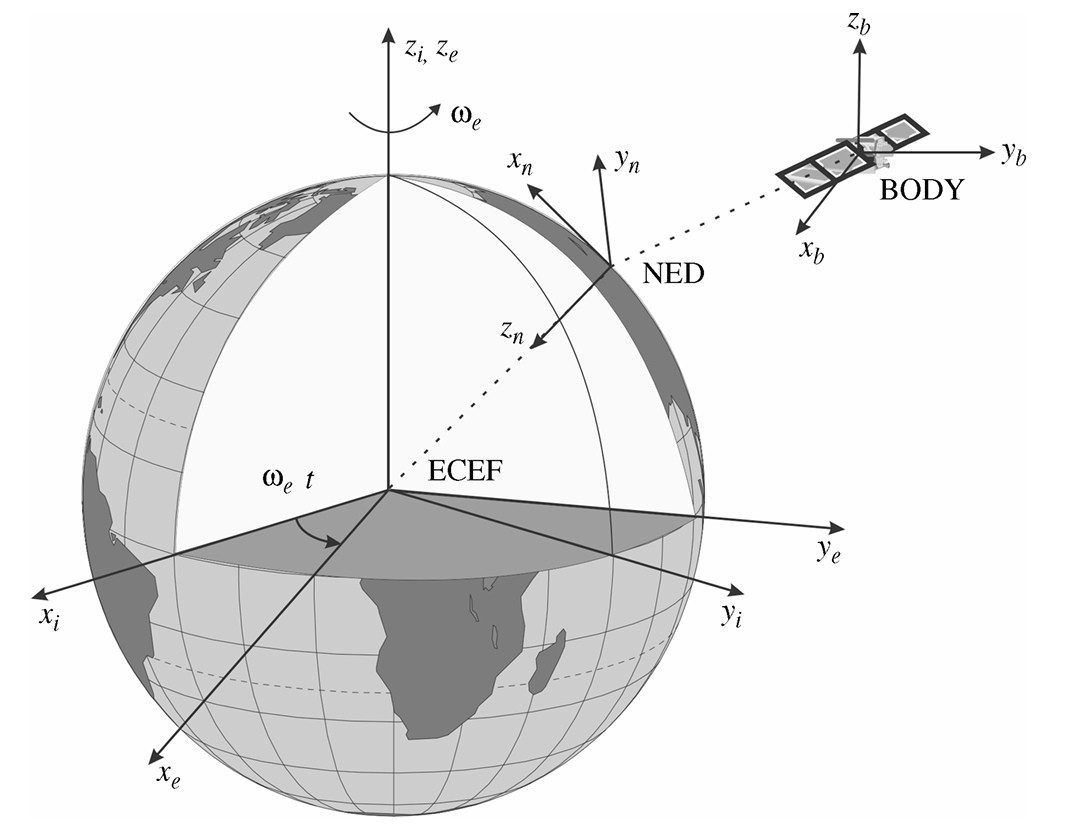
\includegraphics[width=0.6\linewidth]{img/frame.png}};
	\end{tikzpicture}
	
	Earth-Centered reference frames
	\begin{itemize}
		\item ECI - $\{i\}$ - (Earth-centered inertial)
		\item ECEF - $\{e\}$ - (Earth-centered Earth-fixed)
	\end{itemize}
	
	Geographic reference frames
	\begin{itemize}
		\item NED - $\{n\}$ - (North-East-Down)
		\item BODY - $\{b\}$ - (Craft-fixed)
	\end{itemize}
	\vspace{4cm}
	
\end{frame}

% =========================================
% =========================================


\begin{frame}{Fundamental knowledge for modeling}
	\framesubtitle{Coordinates}
	
	
	\begin{tikzpicture}[remember picture,overlay]
		% \node[fill=blue!30, text=white, font=\large, rounded corners] 
		\node at (current page.north east) [xshift=-4cm, yshift=-4.7cm] 
		{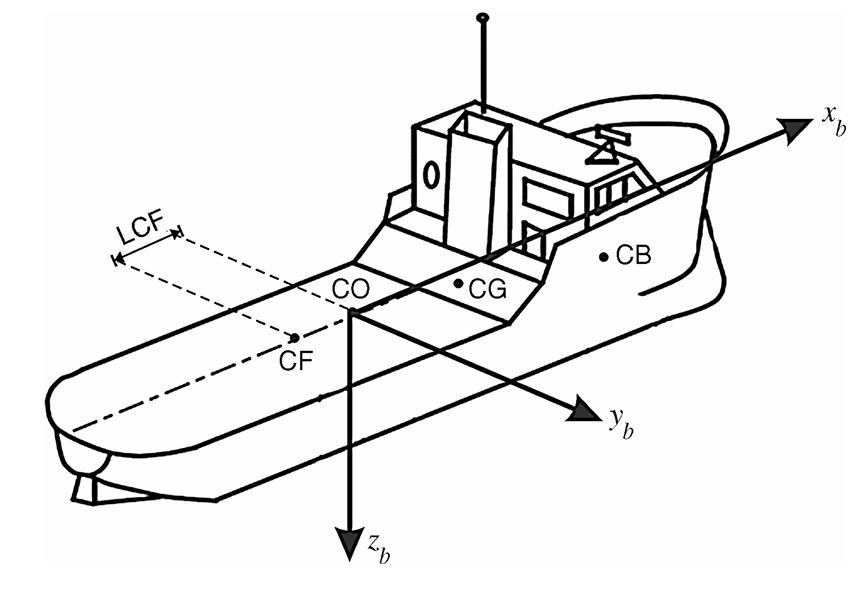
\includegraphics[width=0.65\linewidth]{img/BODY.png}};
	\end{tikzpicture}
	
	The origin of the BODY frame is CO. Then, 
	\begin{itemize}
		\item CG - Center of Gravity
		\item CB - Center of Buoyancy
		\item CF - Center of flotation
	\end{itemize}
	
	\vspace{3cm}
	
	The center of flotation is the centroid of water plane area $A_{wp}$ in calm water.
\end{frame}

% =========================================
% =========================================


\begin{frame}{Fundamental knowledge for modeling}
	\framesubtitle{Notations}
	
	\begin{tikzpicture}[remember picture,overlay]
		% \node[fill=blue!30, text=white, font=\large, rounded corners] 
		\node at (current page.north east) [xshift=-3.8cm, yshift=-3cm] 
		{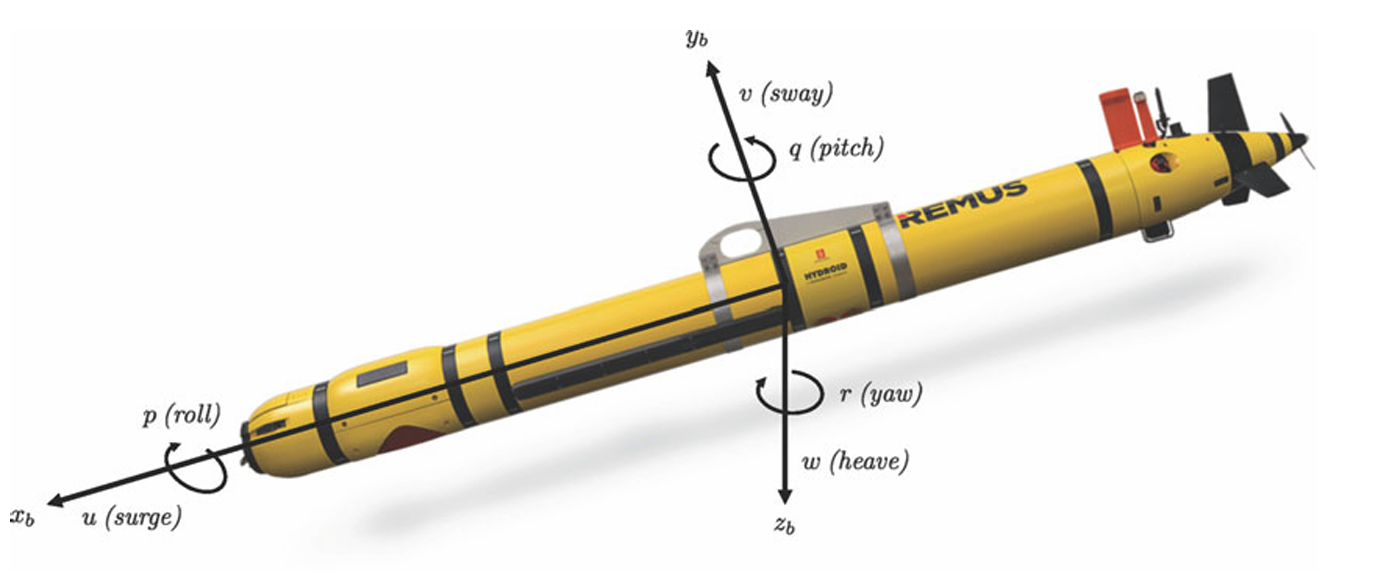
\includegraphics[width=0.7\linewidth]{img/6DOF motion AUV.png}};
	\end{tikzpicture}
	
	\vspace{2cm}
	
	Notation of SNAME (1950)
	\begin{itemize}
		\item Motion of $x$-direction (surge) -- $x$, controlled by $X$ [N]
		\item Motion of $y$-direction (sway) -- $y$, controlled by $Y$ [N]
		\item Motion of $z$-direction (heave) -- $z$, controlled by $Z$ [N]
		\item Rotation of $x$-direction (roll) -- $\phi$, controlled by $K$ [Nm]
		\item Rotation of $y$-direction (pitch) -- $\theta$, controlled by $M$ [Nm]
		\item Rotation of $z$-direction (yaw) -- $\psi$, controlled by $N$ [Nm]
	\end{itemize}
\end{frame}


% =========================================
% =========================================




\begin{frame}{Fundamental knowledge for modeling}
	\framesubtitle{General coordinates}
	
	\begin{tikzpicture}[remember picture,overlay]
		% \node[fill=blue!30, text=white, font=\large, rounded corners] 
		\node at (current page.north east) [xshift=-3.8cm, yshift=-3cm] 
		{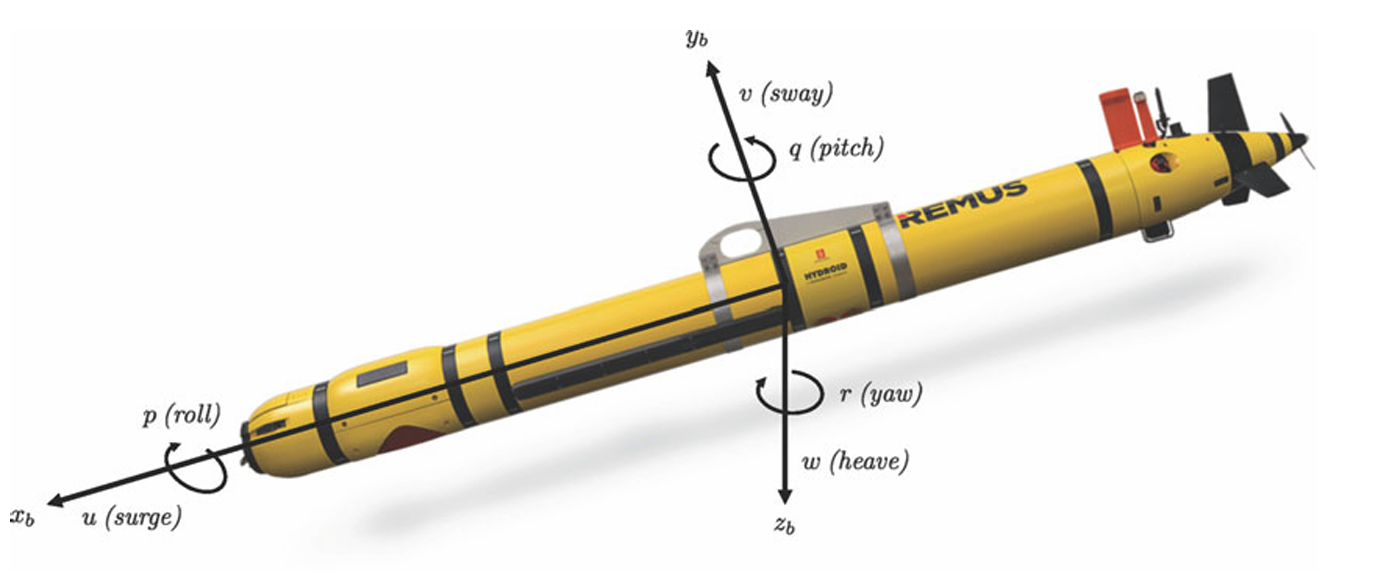
\includegraphics[width=0.7\linewidth]{img/6DOF motion AUV.png}};
	\end{tikzpicture}
	
	\vspace{2cm}
	
	
	General coordinate
	\begin{itemize}
		\item $\eta = \begin{bmatrix}
			(p_{b/n}^n)^\top & \Theta_{nb}^\top
		\end{bmatrix}^\top$, and $p_{b/n}^n = \begin{bmatrix}
			N & E & D
		\end{bmatrix}^\top$, $\Theta_{nb} = \begin{bmatrix}
			\phi & \theta & \psi
		\end{bmatrix}^\top$. In addition, the relative position of craft could be represented in frame ECI.
		\item $\nu = \begin{bmatrix}
			(v_{b/n}^b)^\top & (\omega_{b/n}^b)^\top
		\end{bmatrix}^\top$, and $v_{b/n}^b = \begin{bmatrix}
			u & v & w
		\end{bmatrix}^\top$, $\omega_{b/n}^b = \begin{bmatrix}
			p & q & r
		\end{bmatrix}^\top$
		\item $\tau = \begin{bmatrix}
			\tau_1^\top & \tau_2^\top
		\end{bmatrix}^\top$, and $\tau_1 = \begin{bmatrix}
			X & Y & Z
		\end{bmatrix}^\top$, $\tau_2 = \begin{bmatrix}
			K & M & N
		\end{bmatrix}^\top$
	\end{itemize}
	
	Notice that $\eta$ denotes the position and orientation vector with coordinates in the earth-fix frame. $\nu$ denotes the linear and angular velocity vector with coordinates in the body-fixed frame and $\tau$ denotes the force and torque acting on the vehicle.
	
	
\end{frame}


% =========================================
% =========================================


\begin{frame}{Fundamental knowledge for modeling}
	\framesubtitle{Euler angles}
	
	\begin{tikzpicture}[remember picture,overlay]
		\node at (current page.north east) [xshift=-3cm, yshift=-4.7cm] 
		{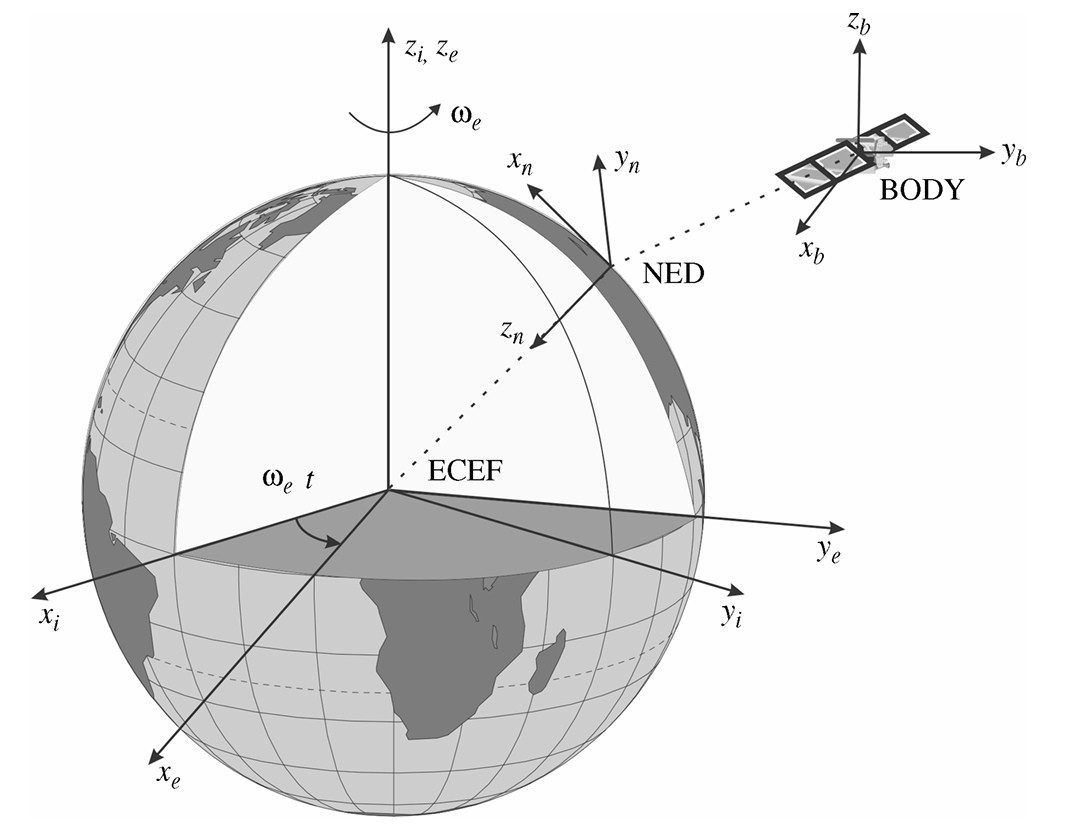
\includegraphics[width=0.5\linewidth]{img/frame.png}};
	\end{tikzpicture}
	
	Frames transformation
	\begin{itemize}
		\item Euler angles
		\item Rotation matrices
		\item Skew-Symmetric of a matrix
		\item Cross product
		\item Euler's theorem on rotation
		\item Linear/Angular velocity transformation
		\item Rotation matrix differential
		\item ...
	\end{itemize}
	
	\vspace{1cm}
	
	In another perspective, \textbf{quaternion} representation is also a good option!
\end{frame}



% =========================================
% =========================================


\begin{frame}{Fundamental knowledge for modeling}
	\framesubtitle{Kinematics}
	The 6 DOFs and 3 DOFs kinematic equations can be expressed in the following
	\begin{block}{6 DOFs kinematic equations}
		\begin{align}
			\dot{\eta} = J_{\Theta}(\eta)\nu
		\end{align}
		that is equivalent to
		\begin{align}
			\begin{bmatrix}
				\dot{p}_{b/n}^n \\ \dot{\Theta}_{nb}
			\end{bmatrix} = \begin{bmatrix}
				R_b^n & 0 \\
				0 & T_{\Theta}(\Theta_{nb})
			\end{bmatrix}\begin{bmatrix}
				v_{b/n}^b \\ \omega_{b/n}^b
			\end{bmatrix}
		\end{align}
		where $R_b^n$ and $T_{\Theta}(\Theta_{nb})$ denote the rotation and transformation matrices.
	\end{block}
	
	\begin{block}{3 DOFs kinematic equations}
		\begin{align}
			\dot{\eta} = R_z(\psi)\nu
		\end{align}
		with $\eta = \begin{bmatrix}
			x & y & \psi
		\end{bmatrix}^\top$ and $\nu = \begin{bmatrix}
			u & v & r
		\end{bmatrix}^\top$
	\end{block}
\end{frame}



% =========================================
% =========================================


\begin{frame}{Fundamental knowledge for modeling}
	\framesubtitle{Other transformations}
	
	In addition, for more purposes, other transformations are needed
	\begin{itemize}
		\item Transformation between ECEF and NED: wide area or terrestrial guidance and navigation.
		\item Transformation between BODY and FLOW: express the hydrodynamic data
	\end{itemize}
	\vspace{4cm}
	
	\begin{tikzpicture}[remember picture,overlay]
		% \node[fill=blue!30, text=white, font=\large, rounded corners] 
		\node at (current page.north west) [xshift=3cm, yshift=-6.5cm] {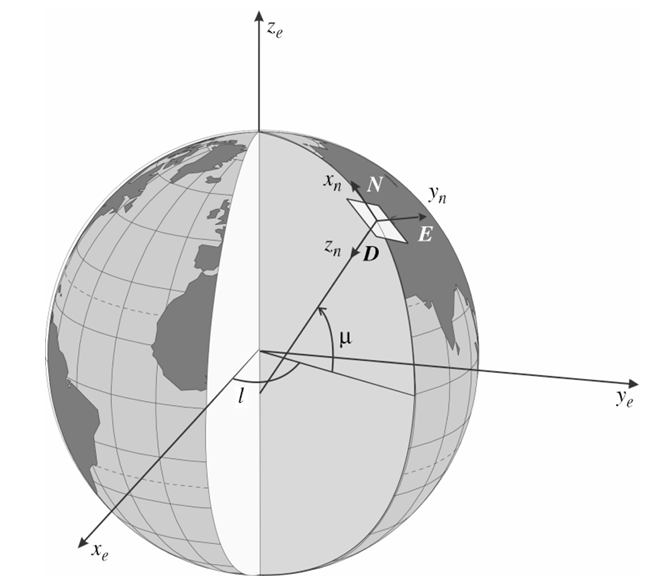
\includegraphics[width=0.4\linewidth]{img/earth surface.png}};
	\end{tikzpicture}
	
	\begin{tikzpicture}[remember picture,overlay]
		% \node[fill=blue!30, text=white, font=\large, rounded corners] 
		\node at (current page.north west) [xshift=8.5cm, yshift=-6.5cm] {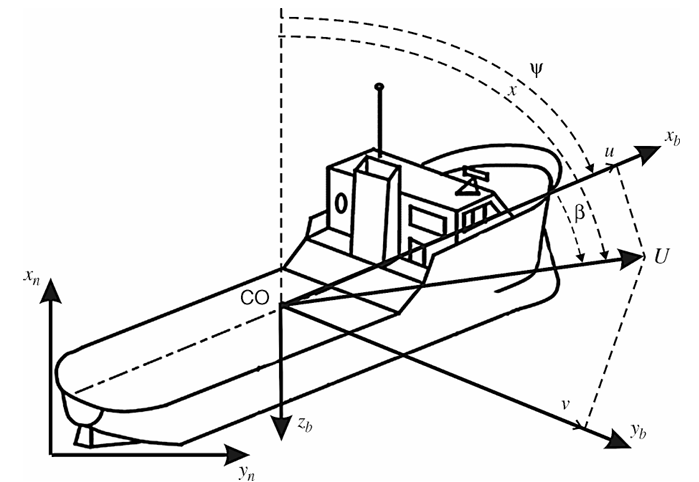
\includegraphics[width=0.5\linewidth]{img/geometrical relationship.png}};
	\end{tikzpicture}
\end{frame}


% =========================================
% =========================================


\begin{frame}{Fundamental knowledge for modeling}
	\framesubtitle{Transformation between BODY and FLOW}
	
	\begin{tikzpicture}[remember picture,overlay]
		% \node[fill=blue!30, text=white, font=\large, rounded corners] 
		\node at (current page.north east) [xshift=-3.8cm, yshift=-3.5cm] 
		{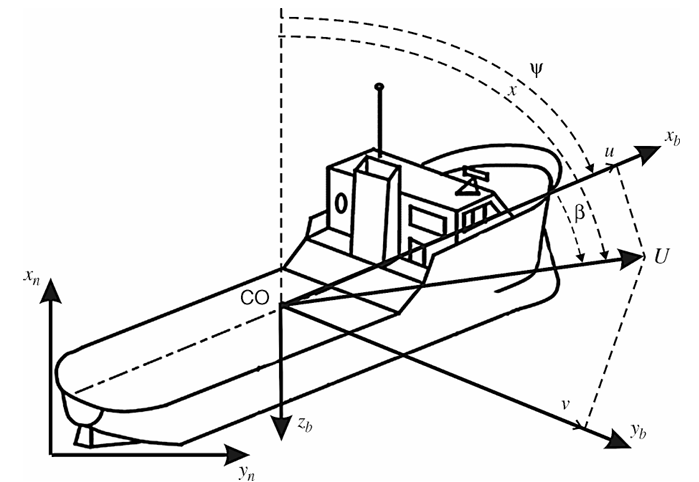
\includegraphics[width=0.5\linewidth]{img/geometrical relationship.png}};
	\end{tikzpicture}
	
	\vspace{1cm}
	
	Similarly, in the first case, the craft \\
	is assumed to be moving on the horizon.
	
	\vspace{0.5cm}
	
	Definition of Course, Heading,\\
	and Sideslip Angles
	\begin{itemize}
		\item Course angle $\chi$: The rotation of $x_n$ and \textbf{velocity vector} $u$ of craft around $z_n$
		\item Heading angle $\psi$: Yaw angle of craft
		\item Sideslip (Drift) angle $\beta$: The rotation of $x_b$ and \textbf{velocity vector} $u$ of craft around $z_b$
	\end{itemize}
	
	Thus $\chi = \psi + \beta$.
	
\end{frame}

% =========================================
% =========================================


\begin{frame}{Fundamental knowledge for modeling}
	\framesubtitle{Transformation between BODY and FLOW} \label{slide: Transformation between BODY and FLOW}
	\begin{tikzpicture}[remember picture,overlay]
		% \node[fill=blue!30, text=white, font=\large, rounded corners] 
		\node at (current page.north east) [xshift=-9.3cm, yshift=-4cm] 
		{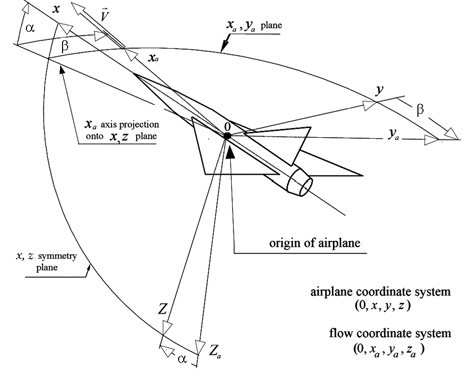
\includegraphics[width=0.55\linewidth]{img/sideslip.png}};
	\end{tikzpicture}
	
	
	\begin{tikzpicture}[remember picture,overlay]
		% \node[fill=blue!30, text=white, font=\large, rounded corners] 
		\node at (current page.north east) [xshift=-3cm, yshift=-3.5cm] 
		{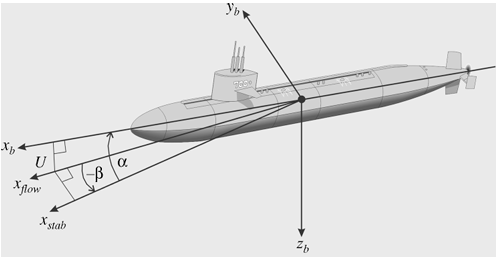
\includegraphics[width=0.5\linewidth]{img/flow UUV.png}};
	\end{tikzpicture}
	
	\vspace{4cm}
	
	\begin{block}{BODY to FLOW transformation}
		\begin{align}
			R_{b}^{flow} = R_{z, -\beta}R_{y, \alpha} = \begin{bmatrix}
				\cos\beta\cos\alpha & \sin\beta & \cos\beta\sin\alpha \\
				-\sin\beta \cos\alpha & \cos\beta & - \sin\beta\sin\alpha \\
				-\sin\alpha & 0 & \cos\alpha
			\end{bmatrix}
		\end{align}
	\end{block}
	
\end{frame}


% =========================================
% =========================================
